\chapter{Fondamentaux de l'ESP32-S3}

\section*{Motivation}

L'objectif de ce TP est de revoir les notions d'acquisition sur microcontrôleur vues en Cours 1. Le traitement numérique du signal exige de maîtriser à la fois la fréquence d'échantillonnage et le temps d'exécution. Ce TP est aussi l'occasion de découvrir les principaux périphériques de l'ESP32-S3 : timers, interruptions, ADC et DMA.\\

Sur une carte comme l'Arduino UNO, les périphériques se configurent en général directement via des registres. Sur une ESP32, nous utiliserons le framework \textbf{Arduino-ESP32}, qui repose sur le framework natif d'Espressif, \textbf{ESP-IDF}, et en simplifie l'usage. L'objectif du TP est donc de comprendre le fonctionnement de ces périphériques et leur configuration au sein de cet écosystème.

\section{ESP32-S3-WROOM-1-N16R8}

L'ESP32-S3 est un microcontrôleur 32 bits double c\oe ur Xtensa LX7. Le module WROOM-1-N16R8 embarque \textbf{16 Mo de mémoire flash} et \textbf{8 Mo de PSRAM} (mémoire vive externe, à ne pas confondre avec la SRAM interne de la puce, limitée à 512 Ko), de quoi couvrir de nombreuses applications embarquées nécessitant de la connectivité. Il dispose de capacités Wi-Fi et Bluetooth Low Energy, ainsi que d'un ensemble de périphériques matériels : GPIO, timers, ADC et contrôleur DMA.\\

\begin{imp}
Trois documents de référence à utiliser : la \href{https://www.mouser.fr/datasheet/3/1574/1/esp32-s3-wroom-1_wroom-1u_datasheet_en.pdf}{datasheet de l'ESP32-S3}, le \href{https://documentation.espressif.com/esp32-s3_technical_reference_manual_en.pdf}{Technical Reference Manual} (TRM), et la \href{https://docs.espressif.com/projects/arduino-esp32/en/latest/getting_started.html}{documentation Arduino-ESP32}.
La datasheet décrit les caractéristiques physiques du composant et le rôle de ses broches ; le TRM détaille l'architecture interne des périphériques et leurs registres ; la documentation Arduino-ESP32 présente les fonctions logicielles et les drivers permettant de les configurer.
\end{imp}

L'ESP32-S3 peut être programmé en \textit{bare-metal}, où le programme pilote directement les ressources matérielles, ou avec un \textit{RTOS} (\textit{Real-Time Operating System}), qui permet notamment de planifier plusieurs tâches. Grâce à son architecture double c\oe ur, l'ESP32-S3 peut également exécuter certaines tâches en parallèle sur ses deux coeurs. Les frameworks que nous utiliserons dans ce module reposent sur FreeRTOS, qui s'occupe notamment de l'ordonnancement des tâches, de leur exécution concurrente sur les deux coeurs, ainsi que de la gestion des mécanismes de synchronisation et de communication entre tâches. FreeRTOS fournit ainsi une couche d'abstraction entre l'application et le matériel, permettant à plusieurs activités de s'exécuter de manière concurrente tout en respectant des priorités et des contraintes temporelles.\\

Le kit électronique de l'ECE inclut une NeuroBoard-S3, une variante de l'ESP32-S3 conçue pour faciliter l'intégration d'une caméra (OV3660) et dotée d'une LED multicolore intégrée ($\texttt{RGB\_LED}$). Son brochage est présenté ci-dessous :

\begin{figure}[!h]
\centering
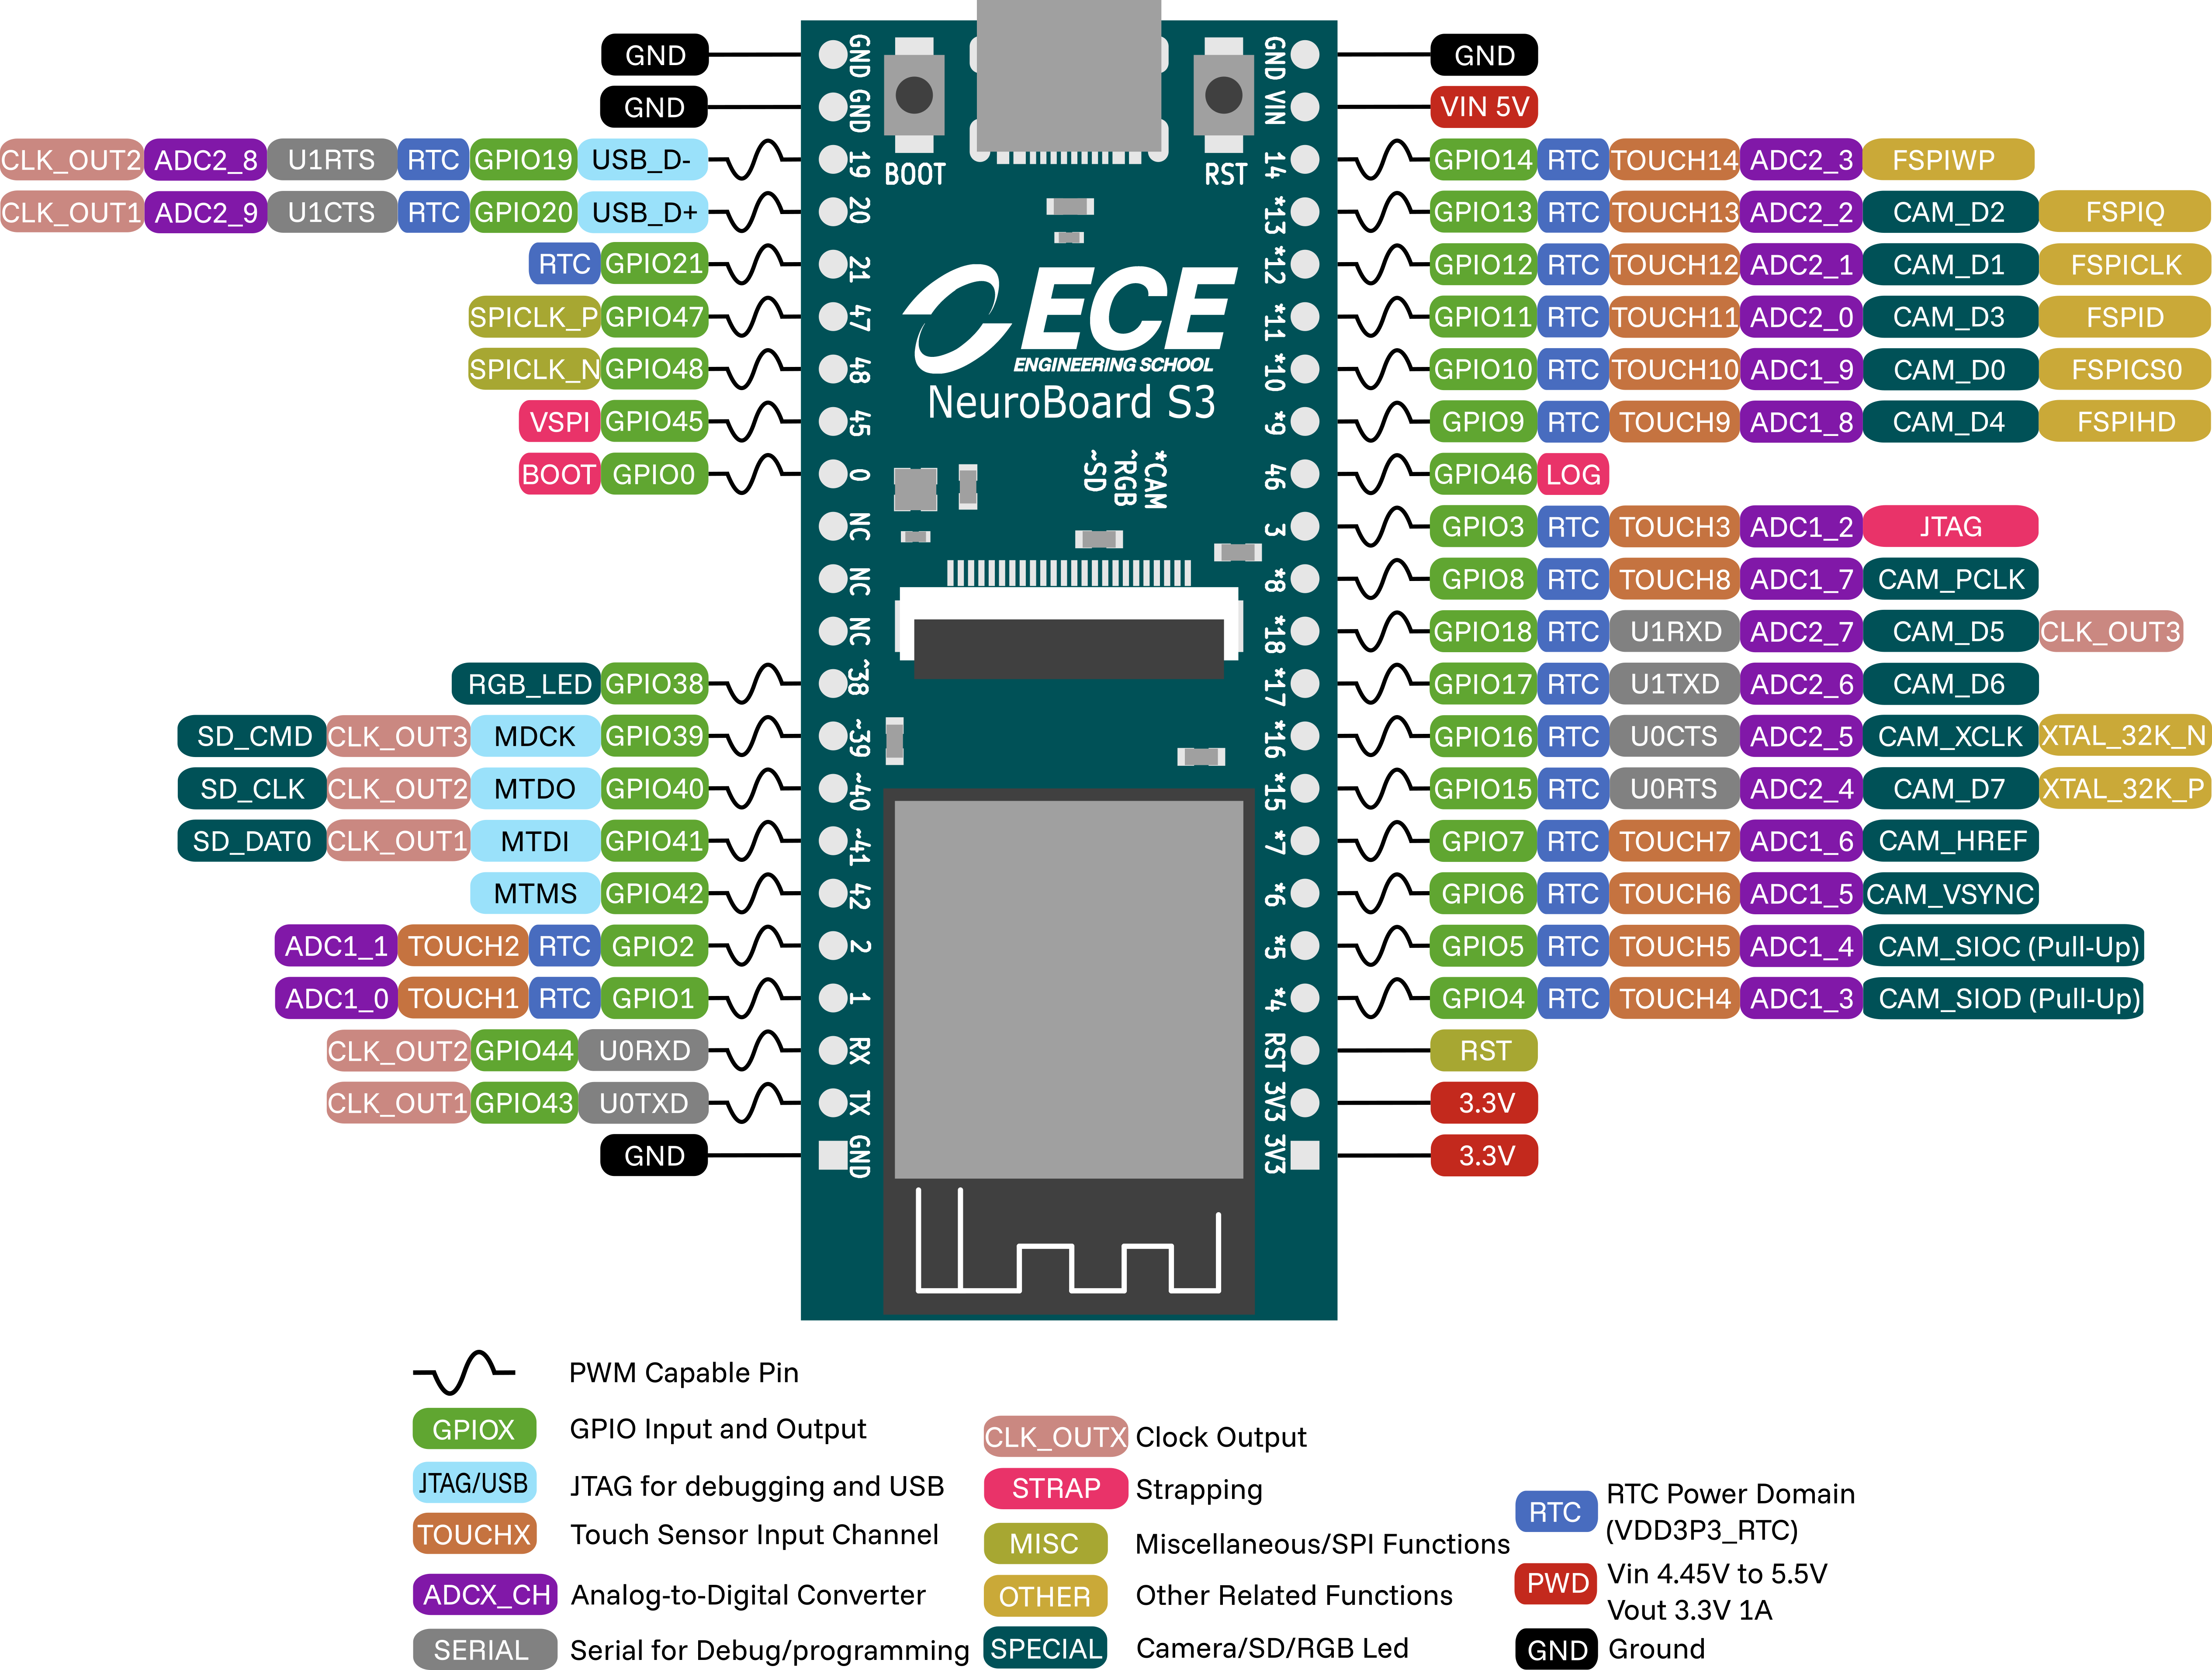
\includegraphics[width=0.7\textwidth]{images/tp0/neuroboard-s3-pinout.png}
\caption{Pinout de la Neuroboard-S3 (ESP32)}
\label{fig:esp32-s3-module-schema}
\end{figure}

\subsection{Écosystèmes de développement : Arduino-ESP32 et ESP-IDF}

Deux frameworks principaux coexistent pour programmer l'ESP32-S3 :\

\textbf{ESP-IDF (\textit{Espressif IoT Development Framework})} : le SDK natif et officiel du fabricant. Écrit en C, il offre un contrôle total sur le silicium, une gestion fine de l'énergie et une intégration native avec FreeRTOS. C'est l'outil de référence pour le développement professionnel et la mise en production, mais sa courbe d'apprentissage est exigeante (configuration CMake, API complexes).\\

\textbf{Arduino-ESP32 (\textit{Arduino Core for ESP32})} : une surcouche logicielle construite \textit{par-dessus} ESP-IDF. Son objectif est de rendre la puce accessible via l'API Arduino familière ($\texttt{void setup()}$, $\texttt{void loop()}$, $\texttt{digitalWrite()}$, etc.). Il est idéal pour le prototypage rapide, car il masque la complexité de la configuration matérielle.\\

\begin{imp}
Dans le cadre du traitement du signal, les fonctions Arduino classiques (comme $\texttt{analogRead()}$) montrent vite leurs limites (fonctions bloquantes, fréquence d'échantillonnage imprécise). Nous utiliserons donc la structure Arduino pour le squelette de nos programmes durant ce module, tout en appelant directement les \textbf{drivers C d'ESP-IDF} (GPTimer, ADC Continuous) dès que performance et contrôle matériel précis seront nécessaires.
\end{imp}

\newpage



\subsubsection{Configuration des interruptions selon le microcontrôleur}

La manière de configurer une interruption dépend du niveau auquel on travaille. On peut soit \textbf{utiliser une abstraction} fournie par le framework Arduino, soit configurer directement le mécanisme d'interruption du microcontrôleur \textbf{selon les registres} d'une carte.\\

L'\textbf{API Arduino} masque une partie des détails matériels. Par exemple, la fonction \texttt{attachInterrupt()} permet d'associer une fonction à une interruption sans avoir à configurer directement les registres du MCU. L'utilisation de \texttt{digitalPinToInterrupt()} convertit le numéro de la broche physique en son identifiant d'interruption matérielle interne, garantissant la portabilité du code entre différentes cartes. Sur l'Arduino UNO classique, \texttt{attachInterrupt()} est disponible sur les GPIO 2 et 3.\\

Le microcontrôleur peut cependant proposer plusieurs mécanismes d'interruption, dont certains ne sont pas directement accessibles à travers cette API. Pour comprendre cette différence, prenons l'exemple de l'Arduino UNO, basée sur l'ATmega328P.

\begin{figure}[!h]
\centering
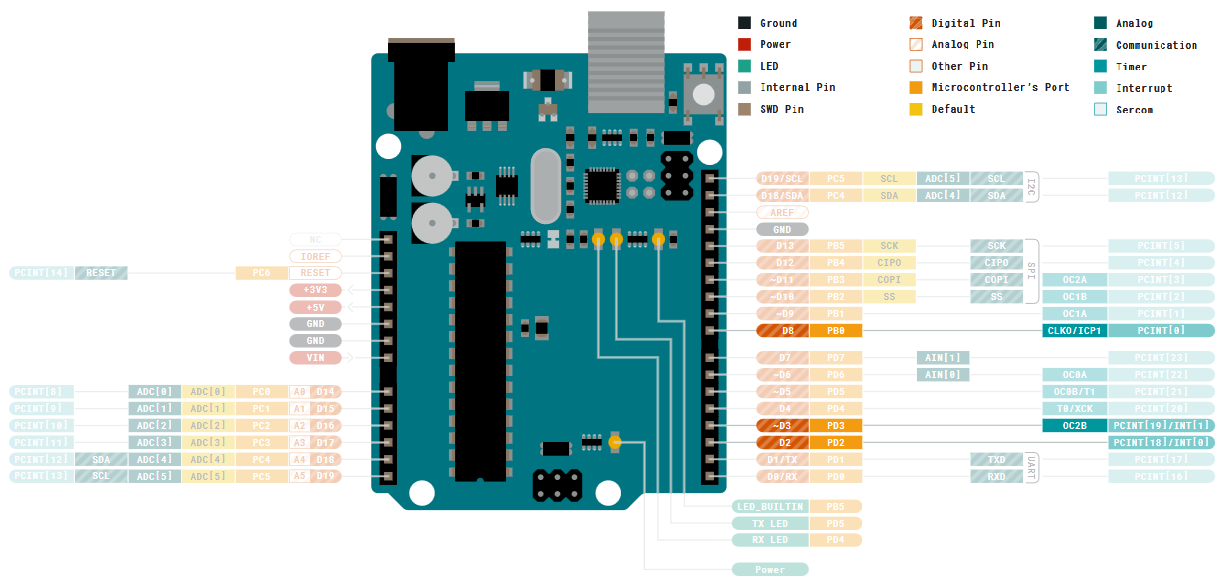
\includegraphics[width=0.9\textwidth]{images/tp0/arduino-pinout.png}
\caption{Pinout de l'Arduino UNO}
\end{figure}

Sur l'ATmega328P, deux mécanismes distincts permettent de détecter un changement sur un pin :\\

Les \textbf{interruptions externes} (\texttt{INT0} et \texttt{INT1}) sont associées à deux broches dédiées du microcontrôleur. Sur l'Arduino UNO, elles correspondent respectivement aux GPIO 2 et 3. Elles peuvent être configurées pour réagir à différents évènements sur la broche, par exemple un front descendant, un front montant ou un niveau bas. Ce sont ces interruptions que l'API Arduino \texttt{attachInterrupt()} permet d'utiliser directement sur l'UNO.\\

Les \textbf{Pin Change Interrupts} (\texttt{PCINT}) reposent sur un autre mécanisme matériel. Elles permettent de surveiller les changements d'état d'un ensemble beaucoup plus large de broches. Par exemple, le GPIO 8 de l'Arduino UNO correspond à \texttt{PB0} sur l'ATmega328P et peut déclencher une \textit{Pin Change Interrupt}. Plusieurs broches partagent alors un même groupe d'interruption (un seul vecteur d'interruption dessert tout le groupe), et des registres dédiés permettent de sélectionner précisément les broches surveillées au sein de ce groupe.\\

Cette différence permet de comprendre l'intérêt de travailler à bas niveau. Avec l'abstraction Arduino, le programme est plus simple et masque les détails propres au microcontrôleur. En revanche, on est limité aux mécanismes et aux broches exposés par cette abstraction. En accédant directement aux registres, on peut utiliser d'autres mécanismes matériels et contrôler précisément leur configuration, au prix d'un code spécifique au microcontrôleur utilisé.\\

Dans le cas de l'Arduino UNO, on peut ainsi comparer les deux approches :\\



\textbf{1. Avec l'abstraction Arduino}\\
Arduino fournit des fonctions qui permettent de configurer facilement une interruption sans avoir à manipuler directement le matériel. Par exemple :

\begin{center}
\texttt{attachInterrupt(digitalPinToInterrupt(BUTTON), buttonISR, FALLING);}
\end{center}

Cette seule ligne permet d'indiquer quelle broche surveiller (BUTTON), quelle fonction exécuter (buttonISR) et sur quel événement déclencher l'interruption (front descendant). Arduino s'occupe ensuite de configurer automatiquement les registres du microcontrôleur.\\

\textbf{2. En configurant directement les registres}\\
Il est également possible de ne pas utiliser ces fonctions Arduino et de configurer directement l'ATmega328P. Dans ce cas, le programmeur doit modifier lui-même certains bits des registres qui contrôlent les interruptions.\\

Pour utiliser une \textit{PCI} sur le GPIO 8, il faut consulter la datasheet de l'ATmega328P afin d'identifier la broche correspondante et les registres à modifier. La datasheet et le pinout indiquent que le GPIO 8 correspond à la broche \texttt{PB0} du microcontrôleur, et que cette broche possède également la fonction \texttt{PCINT0}, c'est-à-dire une entrée d'interruption par changement d'état. Il faut ensuite activer et configurer cette interruption en modifiant les bits des registres concernés à l'aide d'opérations binaires.\\

La différence entre les deux approches est donc principalement le niveau auquel on travaille. Avec Arduino, une fonction comme \texttt{attachInterrupt()} masque la configuration des registres et rend le code plus simple. Avec l'accès direct aux registres, le programmeur doit effectuer lui-même cette configuration, mais il peut contrôler précisément le fonctionnement du microcontrôleur.



Les exemples présentés ci-dessous permettent de comparer ces trois niveaux de programmation :

\begin{center}
\href{https://github.com/Loxed/ece-calcul-embarque-ESP32-2026/blob/main/tp0/code-snippets/button_polling.ino}
{$\texttt{button\_polling.ino}$}
\qquad
\href{https://github.com/Loxed/ece-calcul-embarque-ESP32-2026/blob/main/tp0/code-snippets/button_interrupt_registers.ino}
{$\texttt{button\_interrupt\_registers.ino}$}
\qquad
\href{https://github.com/Loxed/ece-calcul-embarque-ESP32-2026/blob/main/tp0/code-snippets/button_interrupt_abstraction.ino}
{$\texttt{button\_interrupt\_abstraction.ino}$}
\end{center}


\begin{imp}
\textbf{À retenir :} Une abstraction comme \texttt{attachInterrupt()} simplifie l'utilisation des interruptions en masquant leur configuration matérielle. Lorsque l'on travaille directement avec les registres, le code devient spécifique au microcontrôleur, mais il permet d'accéder à des mécanismes matériels supplémentaires et d'en contrôler précisément la configuration.
\end{imp}

\newpage

\subsubsection{Arduino-ESP32 : de l'abstraction Arduino aux drivers ESP-IDF}

Sur un MCU classique comme l'ATmega328P de l'Arduino UNO, on doit accéder directement aux registres pour obtenir un contrôle plus fin du matériel. Sur un ESP32, il existe un niveau intermédiaire entre l'API Arduino (Arduino-ESP32) et les registres : les \textbf{drivers ESP-IDF}.\\

Le framework \textbf{Arduino-ESP32} permet ainsi de retrouver l'approche classique d'Arduino, avec des fonctions comme \texttt{pinMode()}, \texttt{digitalRead()} ou \texttt{attachInterrupt()}, tout en donnant accès aux fonctionnalités plus avancées de l'ESP32 à travers les drivers fournis par ESP-IDF.\\

Ces drivers permettent notamment de configurer plus précisément les périphériques, les timers, les ADC, le DMA ou encore les interruptions, sans avoir à manipuler directement chaque registre du microcontrôleur. Ils constituent donc une abstraction plus proche du matériel, tout en évitant la complexité et la dépendance au matériel qu'impliquerait une configuration registre par registre.\\

On peut ainsi distinguer trois niveaux : l'\textbf{API Arduino}, qui privilégie la simplicité et la portabilité ; les \textbf{drivers ESP-IDF}, qui permettent un contrôle plus fin des périphériques et de leur fonctionnement ; et enfin l'\textbf{accès direct aux registres}, qui offre le niveau de contrôle matériel le plus bas.\\

L'intérêt d'Arduino-ESP32 est donc de pouvoir passer progressivement d'un niveau à l'autre selon les besoins : utiliser les fonctions Arduino pour les opérations courantes, utiliser les drivers ESP-IDF lorsqu'un contrôle plus précis des périphériques ou des interruptions est nécessaire, et accéder directement aux registres uniquement lorsque cela est réellement nécessaire.\\

\begin{imp}
    Votre meilleur ami sera la \href{https://docs.espressif.com/projects/arduino-esp32/en/latest/getting_started.html}{documentation Arduino-ESP32}.
\end{imp}


% \subsubsection{Arduino-ESP32 : L'abstraction matérielle et les drivers ESP-IDF}

% Sur des microcontrôleurs classiques souvent étudiés en débutant (comme l'ATmega328P de l'Arduino UNO), la configuration des périphériques se fait par \textbf{manipulation directe des registres}, comme nous l'avons vu dans l'exemple précédent.\\

% Sur un SoC moderne et très complet comme l'ESP32, la complexité matérielle explose. Configurer manuellement un simple périphérique demanderait de manipuler des dizaines de registres juste pour une simple ISR.\\

% C'est pourquoi nous utiliserons le framework \textbf{Arduino-ESP32}. Il fournit une puissante couche d'abstraction qui s'adapte à nos besoins :
% \begin{itemize}
%     \item \textbf{Les fonctions Arduino classiques :} Pour les opérations courantes, des fonctions familières comme $\texttt{pinMode}$, $\texttt{digitalRead}$ ou $\texttt{attachInterrupt}$ masquent toute la complexité matérielle.
%     \item \textbf{Les drivers ESP-IDF :} Pour les périphériques avancés nécessitant un contrôle précis (Timers matériels, ADC continu, DMA), Arduino-ESP32 donne un accès direct aux drivers C natifs d'Espressif (ESP-IDF). Ces drivers créent une couche d'abstraction de haut niveau par rapport aux registres, tout en garantissant des performances optimales.
% \end{itemize}

% \begin{imp}
% \textbf{Le rôle d'Arduino-ESP32 :} Il agit comme un pont. Il permet de prototyper rapidement avec la syntaxe Arduino, tout en offrant la puissance des drivers ESP-IDF dès que les besoins en traitement du signal ou en gestion du temps deviennent exigeants.
% \end{imp}



\section{Configuration des Timers/Counters}

Les \textbf{Timers/Counters} sont des périphériques matériels dédiés au comptage du temps. Contrairement à une fonction comme \texttt{millis()}, qui fournit directement une mesure du temps utilisable par le programme, un timer matériel possède son propre compteur qui évolue automatiquement à partir d'une horloge. Il peut ensuite déclencher une alarme lorsqu'une valeur est atteinte et provoquer une interruption. Ce mécanisme permet ainsi une gestion du temps beaucoup plus précise et indépendante de l'exécution du programme principal. À l'inverse, une mesure réalisée avec \texttt{millis()} dans une boucle en polling dépend de la durée d'exécution des autres instructions de la boucle, ce qui peut introduire un délai entre le moment où la durée est effectivement atteinte et celui où elle est détectée.\\

Le compteur n'avance pas nécessairement à chaque cycle de l'horloge du microcontrôleur. Un \textbf{prescaler} permet de diviser la fréquence de l'horloge avant qu'elle n'alimente le compteur. On peut ainsi choisir une fréquence de comptage adaptée au besoin. Par exemple, avec une fréquence de comptage de $1 MHz$, chaque incrément du compteur correspond à $1 \mu s$. Une alarme réglée à 1000 ticks déclenchera alors un événement toutes les $1ms$.\\

Sur l'\textbf{ESP32-S3}, quatre timers matériels génériques sont disponibles. Ils utilisent des compteurs de \textbf{64 bits} et des prescalers de \textbf{16 bits}. Les timers peuvent fonctionner avec différentes sources d'horloge, notamment l'horloge APB ou l'oscillateur quartz de $40 MHz$. \\

Ces caractéristiques peuvent être retrouvées dans la documentation matérielle et dans le driver fourni par Espressif. L'intérêt est justement de ne pas avoir à manipuler directement les registres du timer : le driver permet d'accéder à ces fonctionnalités à travers une API.\\

Avec \textbf{Arduino-ESP32}, cette configuration est fortement simplifiée. Par exemple, \texttt{timerBegin(1000000)} configure un timer avec une fréquence de comptage de $1,\mathrm{MHz}$. Une interruption peut ensuite être associée avec \texttt{timerAttachInterrupt()}, et une alarme avec \texttt{timerAlarm()}. Le paramètre d'alarme correspond alors directement au nombre de ticks avant le déclenchement. \cite{arduino_timer} \\

Avec \textbf{ESP-IDF}, on travaille à un niveau plus proche du matériel. Le driver \texttt{GPTimer} permet notamment de choisir la source d'horloge, la résolution du compteur, son sens de comptage, la valeur de l'alarme, l'auto-rechargement ainsi que certains paramètres liés à l'interruption. Il est également possible d'associer une callback à l'événement d'alarme. \cite{esp32s3_gptimer} \\

On retrouve donc ici la même organisation que pour les interruptions : \textbf{Arduino-ESP32} fournit une abstraction simple pour les besoins courants, tandis que les \textbf{drivers ESP-IDF} donnent davantage de contrôle sur le périphérique sans nécessiter de configurer directement chaque registre. La lecture de la documentation ESP-IDF permet ainsi de comprendre quelles possibilités matérielles sont réellement disponibles derrière l'API Arduino.\\

% {https://github.com/Loxed/ece-calcul-embarque-ESP32-2026/blob/main/tp0/code-snippets/esp32_timer_interrupt.ino}{}

Un exemple complet est disponible dans la documentation officielle Arduino-ESP32 : \href{https://docs.espressif.com/projects/arduino-esp32/en/latest/api/timer.html}{$\texttt{Arduino\text{-}ESP32\ Timer\ API}$}. La documentation du driver GPTimer d'ESP-IDF détaille quant à elle la configuration matérielle accessible à travers ce niveau d'abstraction : \href{https://docs.espressif.com/projects/esp-idf/en/latest/esp32s3/api-reference/peripherals/gptimer.html}{$\texttt{ESP\text{-}IDF\ GPTimer}$}. \cite{arduino_timer,esp32s3_gptimer}\


\RepoLink{tp0/code-snippets/esp32_timer_interrupt.ino}{Code de l'interruption timer}


% \subsection{Configuration des Timers/Counters}

% % Expliquer les Timer Coutner pour avoir plus de precision sur le temps que millis() et compagnie

% les prescalers threshold etc..

% % Expliquer GPTimer de ESP-IDF / Arduino-ESP32.

% % provide un exemple sur github / en lien

% % Cette reference cestspecifique a ESP-IDF. ya forcement d es trucs pour Arduino ESP32
% % Référence : \href{https://docs.espressif.com/projects/esp-idf/en/latest/esp32s3/api-reference/peripherals/gptimer.html}{ESP-IDF - GPTimer}

% % https://docs.espressif.com/projects/arduino-esp32/en/latest/api/timer.html

% % on a une ESP32-S3. explique le nombre d e timers, leur frequence / caracteristiques / prescale etc..








\newpage



\section{Configuration de l'ADC}

L'\textbf{ADC} (\textit{Analog-to-Digital Converter}) est le périphérique qui convertit une tension analogique, par exemple la sortie d'un capteur, en une valeur numérique exploitable par le processeur. C'est un élément fondamental pour toute application d'acquisition et de traitement du signal.

\subsection{Limites de l'API Arduino}

Sur un microcontrôleur comme l'ESP32, l'API Arduino-ESP32 propose la fonction classique \texttt{analogRead()}. Son utilisation est particulièrement simple :

\begin{verbatim}
int valeur = analogRead(mon_pin);
\end{verbatim}

Cependant, cette simplicité masque un défaut majeur pour nos applications : cette fonction est \textbf{bloquante et imprécise}. Lorsqu'elle est appelée, le CPU attend la fin de la conversion avant de poursuivre l'exécution du programme. Il devient alors impossible de garantir une fréquence d'échantillonnage stable, car le temps de conversion ainsi que la durée d'exécution des autres instructions de la boucle s'ajoutent au délai.\\

Pour du prototypage rapide, cette approche est acceptable. En revanche, pour une application de traitement du signal nécessitant une fréquence d'échantillonnage précise, elle devient problématique.

\subsection{Le mode continu (DMA) du driver ESP-IDF}

Pour une acquisition performante et précise, nous allons utiliser le driver \textbf{ADC en mode continu} d'ESP-IDF, accessible via \texttt{esp\_adc/adc\_continuous.h}. Ce mode de fonctionnement déporte l'effort d'acquisition vers le matériel :

\begin{enumerate}
    \item Un \textbf{timer} interne déclenche les conversions à une fréquence d'échantillonnage configurée avec précision.
    \item Les résultats sont transférés de l'ADC vers une zone de la mémoire vive (SRAM) par le contrôleur \textbf{DMA}, sans intervention du CPU pour chaque échantillon.
    \item Le CPU, libéré de ces tâches répétitives, peut se consacrer à d'autres opérations, comme les calculs ou la gestion des communications, puis lire les échantillons par blocs lorsqu'ils sont disponibles.
\end{enumerate}

C'est ce mécanisme qui permet d'atteindre des fréquences d'échantillonnage élevées et stables, essentielles en traitement numérique du signal.

\subsection{Configuration et mise en oeuvre}

La configuration du driver se déroule en trois étapes, que l'on retrouve dans la fonction \texttt{setup()} du programme Arduino :

\begin{enumerate}
    \item \textbf{Allocation des ressources :} on initialise le driver en lui allouant un tampon mémoire interne et en définissant la taille d'une trame de conversion. Le driver réserve alors les ressources matérielles nécessaires, notamment celles utilisées pour le transfert DMA.
    
    \item \textbf{Configuration du canal :} on définit le ou les canaux de l'ADC à échantillonner, avec leur résolution, par exemple 12 bits, ainsi que leur atténuation d'entrée afin d'adapter la plage de tension mesurable au signal.
    
    \item \textbf{Démarrage de l'acquisition :} une fois le driver configuré et démarré, le matériel échantillonne en continu de manière autonome.
\end{enumerate}

La lecture des données se fait ensuite dans la fonction \texttt{loop()}, indépendamment du rythme de l'acquisition :

\begin{verbatim}
#include "esp_adc/adc_continuous.h"

#define ADC_UNIT        ADC_UNIT_1
#define ADC_CHANNEL     ADC_CHANNEL_4     // Correspond à un GPIO précis
#define SAMPLE_FREQ_HZ  20000             // 20 kHz d'échantillonnage
#define CONV_FRAME_SIZE 256               // Taille d'une trame, en octets

adc_continuous_handle_t adc_handle = NULL;

void setup() {
    Serial.begin(115200);

    // 1. Allocation des ressources du driver
    adc_continuous_handle_cfg_t adc_config = {
        .max_store_buf_size = 1024,
        .conv_frame_size = CONV_FRAME_SIZE,
    };
    ESP_ERROR_CHECK(adc_continuous_new_handle(&adc_config, &adc_handle));

    // 2. Configuration du canal à échantillonner
    adc_digi_pattern_config_t adc_pattern = {
        .atten = ADC_ATTEN_DB_12,
        .channel = ADC_CHANNEL,
        .unit = ADC_UNIT,
        .bit_width = ADC_BITWIDTH_12,
    };

    adc_continuous_config_t dig_cfg = {
        .pattern_num = 1,
        .adc_pattern = &adc_pattern,
        .sample_freq_hz = SAMPLE_FREQ_HZ,
        .conv_mode = ADC_CONV_SINGLE_UNIT_1,
        .format = ADC_DIGI_OUTPUT_FORMAT_TYPE2,
    };
    ESP_ERROR_CHECK(adc_continuous_config(adc_handle, &dig_cfg));

    // 3. Démarrage de l'acquisition
    ESP_ERROR_CHECK(adc_continuous_start(adc_handle));
}

void loop() {
    adc_continuous_data_t samples[64];
    uint32_t num_samples = 0;

    // Lecture des échantillons déjà accumulés par le driver.
    // La fonction est bloquante au maximum 100 ms si aucun
    // échantillon n'est disponible.
    esp_err_t ret = adc_continuous_read_parse(
        adc_handle,
        samples,
        64,
        &num_samples,
        100
    );

    if (ret == ESP_OK) {
        for (int i = 0; i < num_samples; i++) {
            if (samples[i].valid) {
                Serial.printf(
                    "Canal %d : %lu\n",
                    samples[i].channel,
                    samples[i].raw_data
                );
            }
        }
    }
}
\end{verbatim}

\begin{imp}
Dans ce code, la DMA n'est jamais configurée explicitement. C'est la fonction \texttt{adc\_continuous\_new\_handle()} qui s'occupe en interne de réserver les ressources DMA et d'allouer les tampons nécessaires. Le driver ESP-IDF fournit ainsi une abstraction de plus haut niveau qui encapsule la complexité de la configuration matérielle.
\end{imp}

\begin{imp}
\textbf{À retenir :} pour une acquisition précise et non bloquante, on délaisse \texttt{analogRead()} au profit du driver \textbf{ADC continu} d'ESP-IDF. Ce dernier s'appuie sur le matériel pour échantillonner à une fréquence fixe et transférer les données en mémoire de manière autonome, laissant ainsi le CPU libre pour d'autres tâches.
\end{imp}

Un exemple complet est disponible dans la documentation officielle Arduino-ESP32 : \href{https://docs.espressif.com/projects/arduino-esp32/en/latest/api/adc.html}{\texttt{Arduino-ESP32 ADC API}}. La documentation du driver ADC continu d'ESP-IDF détaille quant à elle les options de configuration plus avancées : \href{https://docs.espressif.com/projects/esp-idf/en/latest/esp32s3/api-reference/peripherals/adc_continuous.html}{\texttt{ESP-IDF ADC Continuous Mode Driver}}. \cite{arduino_adc,esp32s3_adc_continuous}

\RepoLink{tp0/code-snippets/esp32\_adc\_continuous.ino}{Code de l'acquisition ADC continue}

\section{Fonctionnement de la DMA}

Contrairement aux GPIO, aux timers ou à l'ADC, la DMA (\textit{Direct Memory Access}) n'est pas un périphérique que l'on configure nécessairement de manière directe et isolée. Il s'agit d'un \textbf{mécanisme matériel de transfert} dont le rôle est de déplacer des données entre la mémoire et un périphérique sans intervention du CPU une fois le transfert initié.

\begin{imp}
Arduino-ESP32 n'expose \textbf{aucune API générique de configuration de la DMA}. Celle-ci est utilisée en interne par certains drivers ESP-IDF, notamment pour l'ADC continu, l'I2S ou le SPI, afin de transférer des données à haute fréquence sans monopoliser le CPU. On ne configure donc généralement pas la DMA ``toute seule'' : on utilise un périphérique et son driver qui s'appuient sur ce mécanisme.
\end{imp}

Dans le cadre de ce TP, c'est le driver \textbf{ADC en mode continu}, présenté dans la section précédente, qui nous intéresse. Sur les architectures ESP32 concernées, le mécanisme d'acquisition numérique s'appuie sur des ressources matérielles dédiées et sur la DMA afin de transférer automatiquement les échantillons ADC vers la mémoire à une fréquence constante.

Le principe général est donc le suivant :

\begin{enumerate}
    \item L'ADC effectue les conversions à la fréquence d'échantillonnage configurée.
    \item Les résultats sont placés dans une mémoire tampon par le mécanisme DMA.
    \item Le CPU récupère les données par blocs lorsqu'elles sont disponibles.
\end{enumerate}

Le CPU n'a ainsi pas besoin de lire chaque échantillon individuellement, contrairement à une utilisation classique de \texttt{analogRead()}. Cette architecture permet d'obtenir une acquisition plus régulière et de consacrer les ressources processeur au traitement des données acquises.